%----------------------------------------------------------------------------------------
%    PACKAGES AND THEMES
%----------------------------------------------------------------------------------------

\documentclass[aspectratio=169,xcolor=dvipsnames]{beamer}
\usetheme{SimpleDarkBlue}

\usepackage{hyperref}
\usepackage{graphicx} % Allows including images
\usepackage{booktabs} % Allows the use of \toprule, \midrule and \bottomrule in tables
\usepackage{xfrac}
\usepackage{mathtools}
\usepackage{subcaption}
\usepackage{siunitx}
\usepackage{amsmath}
\usepackage{amssymb}
\usepackage[LGR,T1]{fontenc}


\newcommand{\half}{$\sfrac{1}{2}$ }
\newcommand{\pauliz}{\begin{pmatrix}
    1 & 0 \\
    0 & -1 
    \end{pmatrix}}
\newcommand{\halfpi}{\frac{\pi}{2}}
\newcommand{\Bnot}{\vec{B}_0}
\newcommand{\Bone}{\vec{B}_1}


\DeclarePairedDelimiter\bra{\langle}{\rvert}
\DeclarePairedDelimiter\ket{\lvert}{\rangle}
\DeclarePairedDelimiterX\braket[2]{\langle}{\rangle}{#1\,\delimsize\vert\,\mathopen{}#2}
\DeclareMathAlphabet{\mathgtt}{LGR}{cmtt}{m}{n}

%----------------------------------------------------------------------------------------
%    TITLE PAGE
%----------------------------------------------------------------------------------------

\title{Nuclear Magnetic Resonance (NMR)}
\subtitle{A Brief Introduction and Applications}

\author{Ali Ahmed \and Neil Mandar \and Zain Kamal}

\institute
{
    Department of Physcis \& Astronomy, Rutgers University % Your institution for the title page
}
\date{\today} % Date, can be changed to a custom date

%----------------------------------------------------------------------------------------
%    PRESENTATION SLIDES
%----------------------------------------------------------------------------------------

\begin{document}

\begin{frame}
    % Print the title page as the first slide
    \titlepage
\end{frame}

\begin{frame}{Overview}
    % Throughout your presentation, if you choose to use \section{} and \subsection{} commands, these will automatically be printed on this slide as an overview of your presentation
    \tableofcontents
\end{frame}

%------------------------------------------------
\section{Principles of NMR}
%------------------------------------------------

\begin{frame}{Setup}
    

    \begin{minipage}{0.4\linewidth}
        \begin{figure}
            \centering
            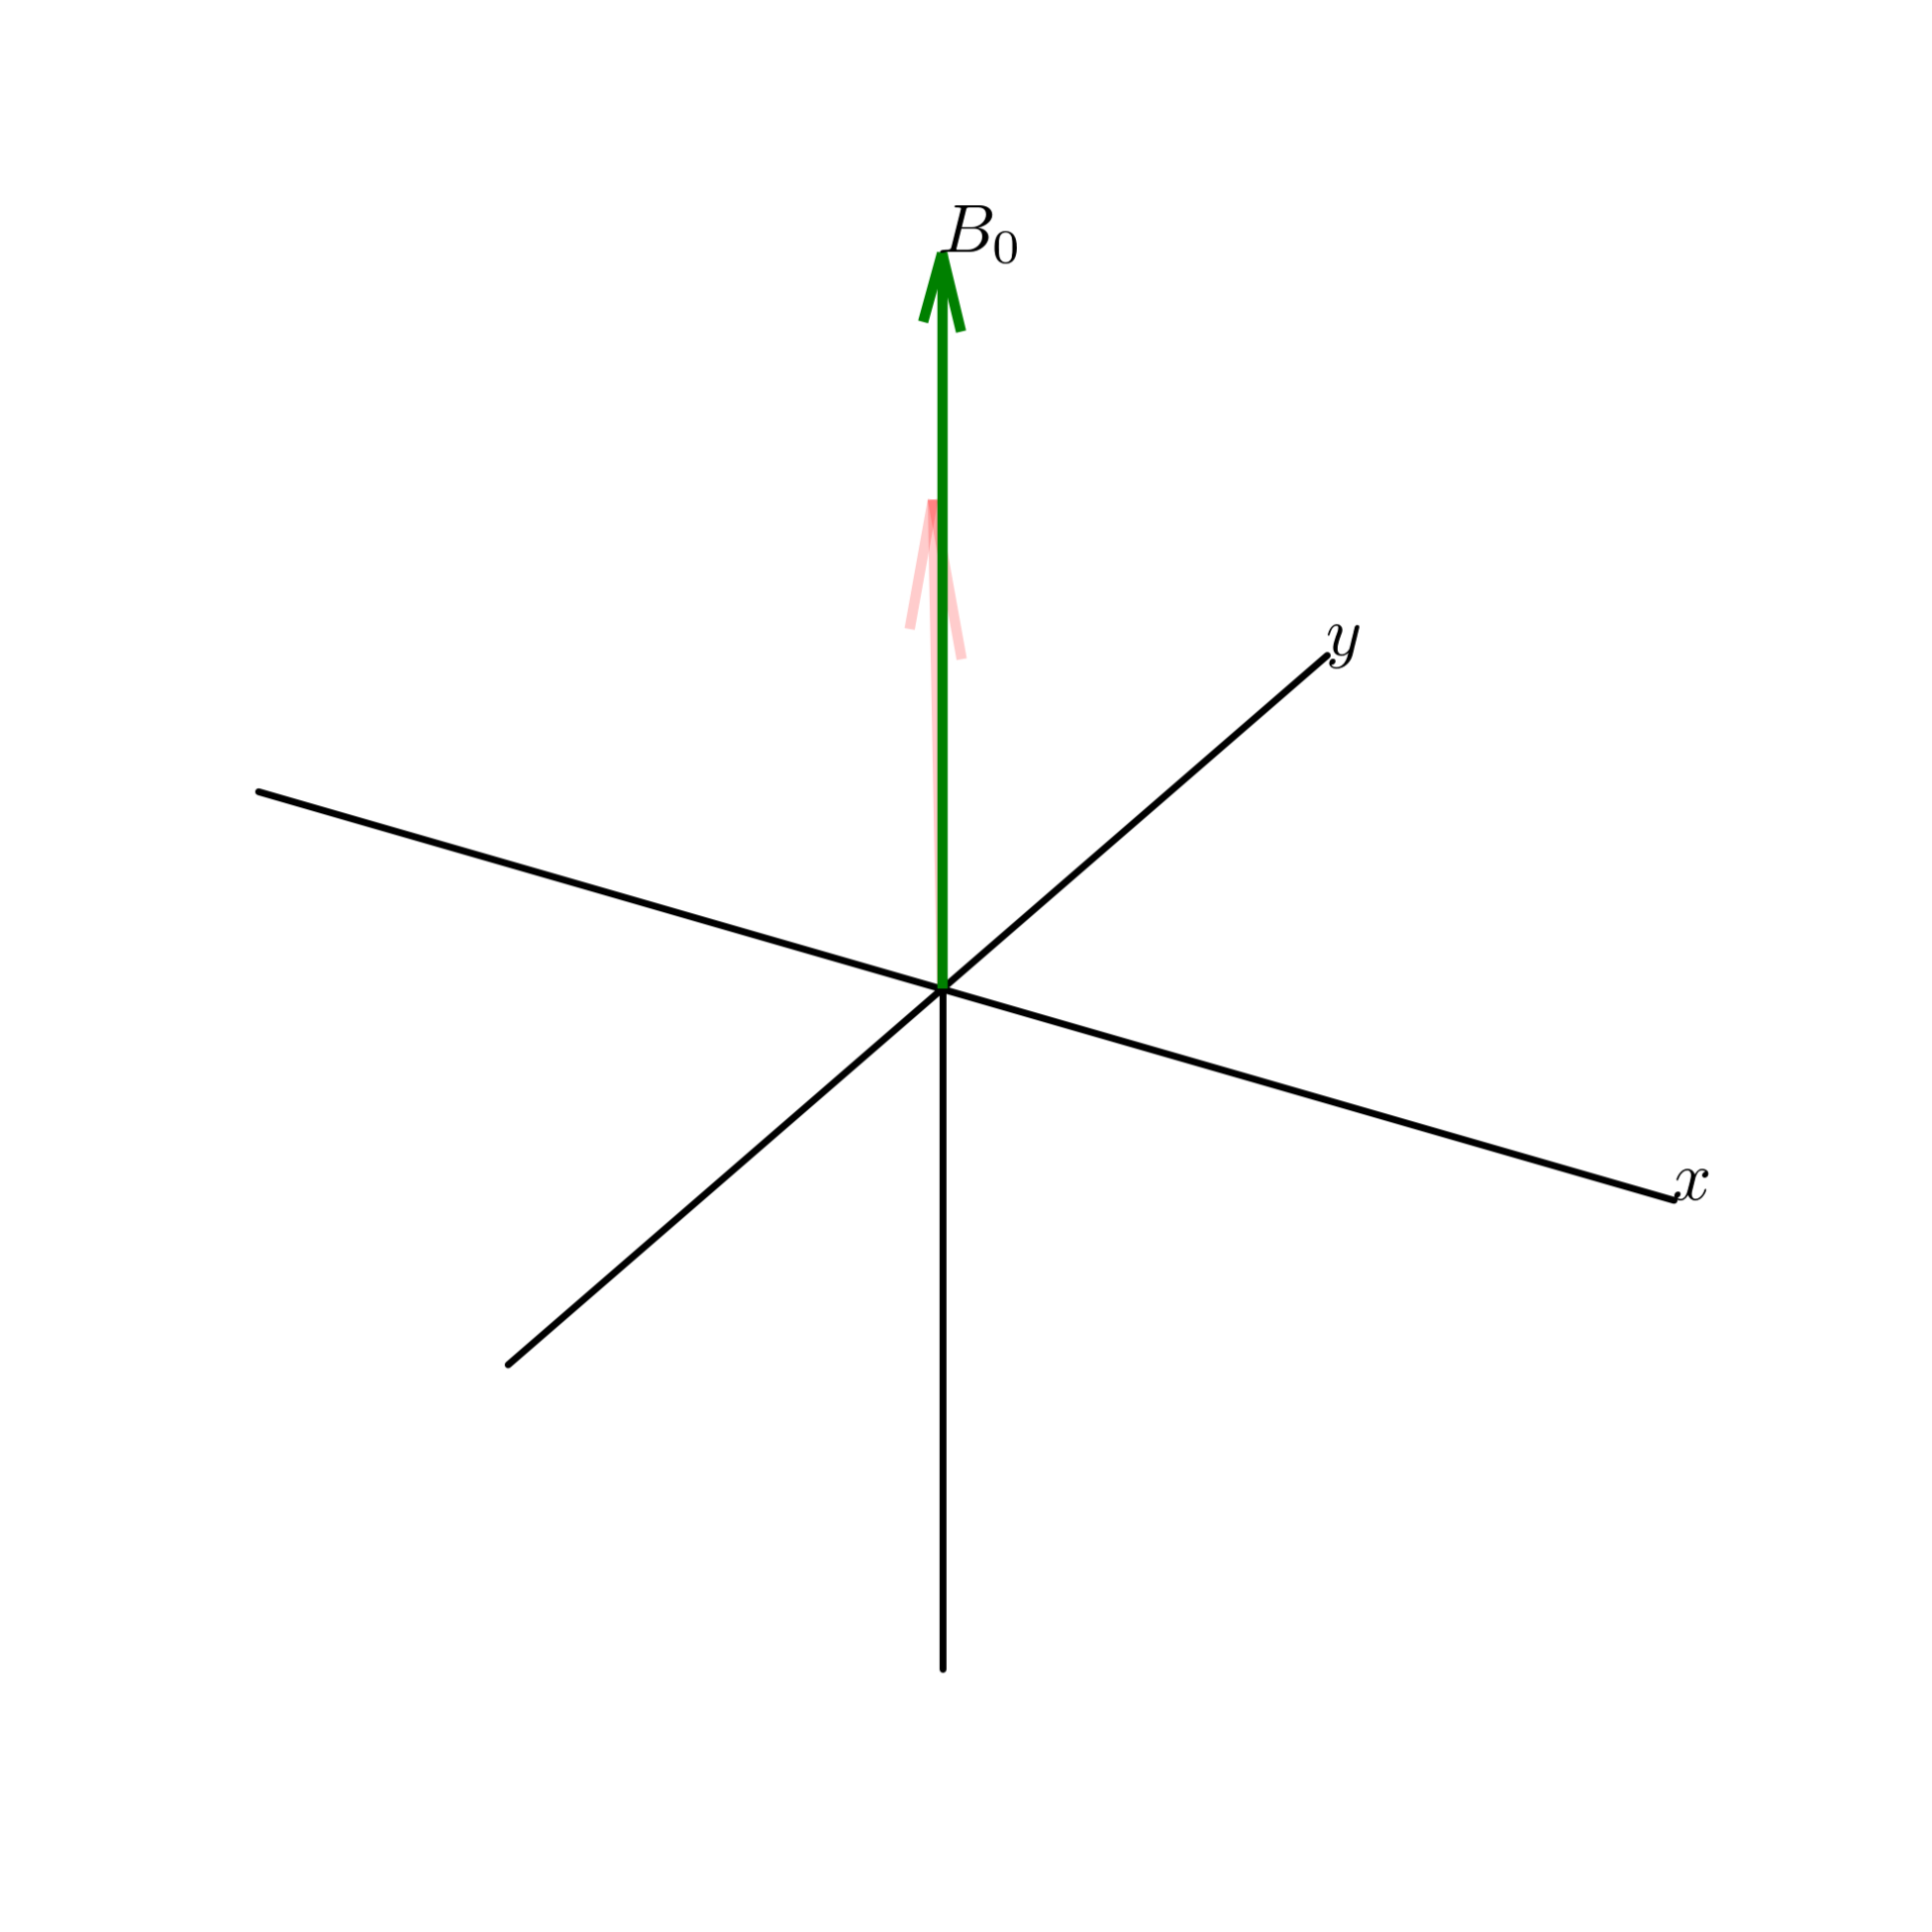
\includegraphics[width = \linewidth]{setup.png}\\
            \caption{Typical $\Bnot$ and vector aligned with field}
        \end{figure}
    \end{minipage}
    \hfill
    \begin{minipage}{0.5\linewidth}
        \begin{itemize}
            \item Spin \half nuclei 
            \item Strong magnetic field, denoted $\Bnot$
        \end{itemize}
        \begin{block}{Energy and Hamiltonian}
            Magnetic moment of nucleus
            \begin{equation}
                \vec{\mu} = \gamma \vec{S}
            \end{equation}
            Yields energy and Hamiltonian of 
            \begin{equation}
                E = -\vec{\mu} \cdot \vec{B_0}
            \end{equation}
            \begin{equation}\label{eqn:base-hamiltonian}
                H = -\gamma \vec{B_0} \cdot S
            \end{equation}
        \end{block}
    \end{minipage}
    
    % \begin{tabular}{cl}
    %     \begin{tabular}{c}
    %             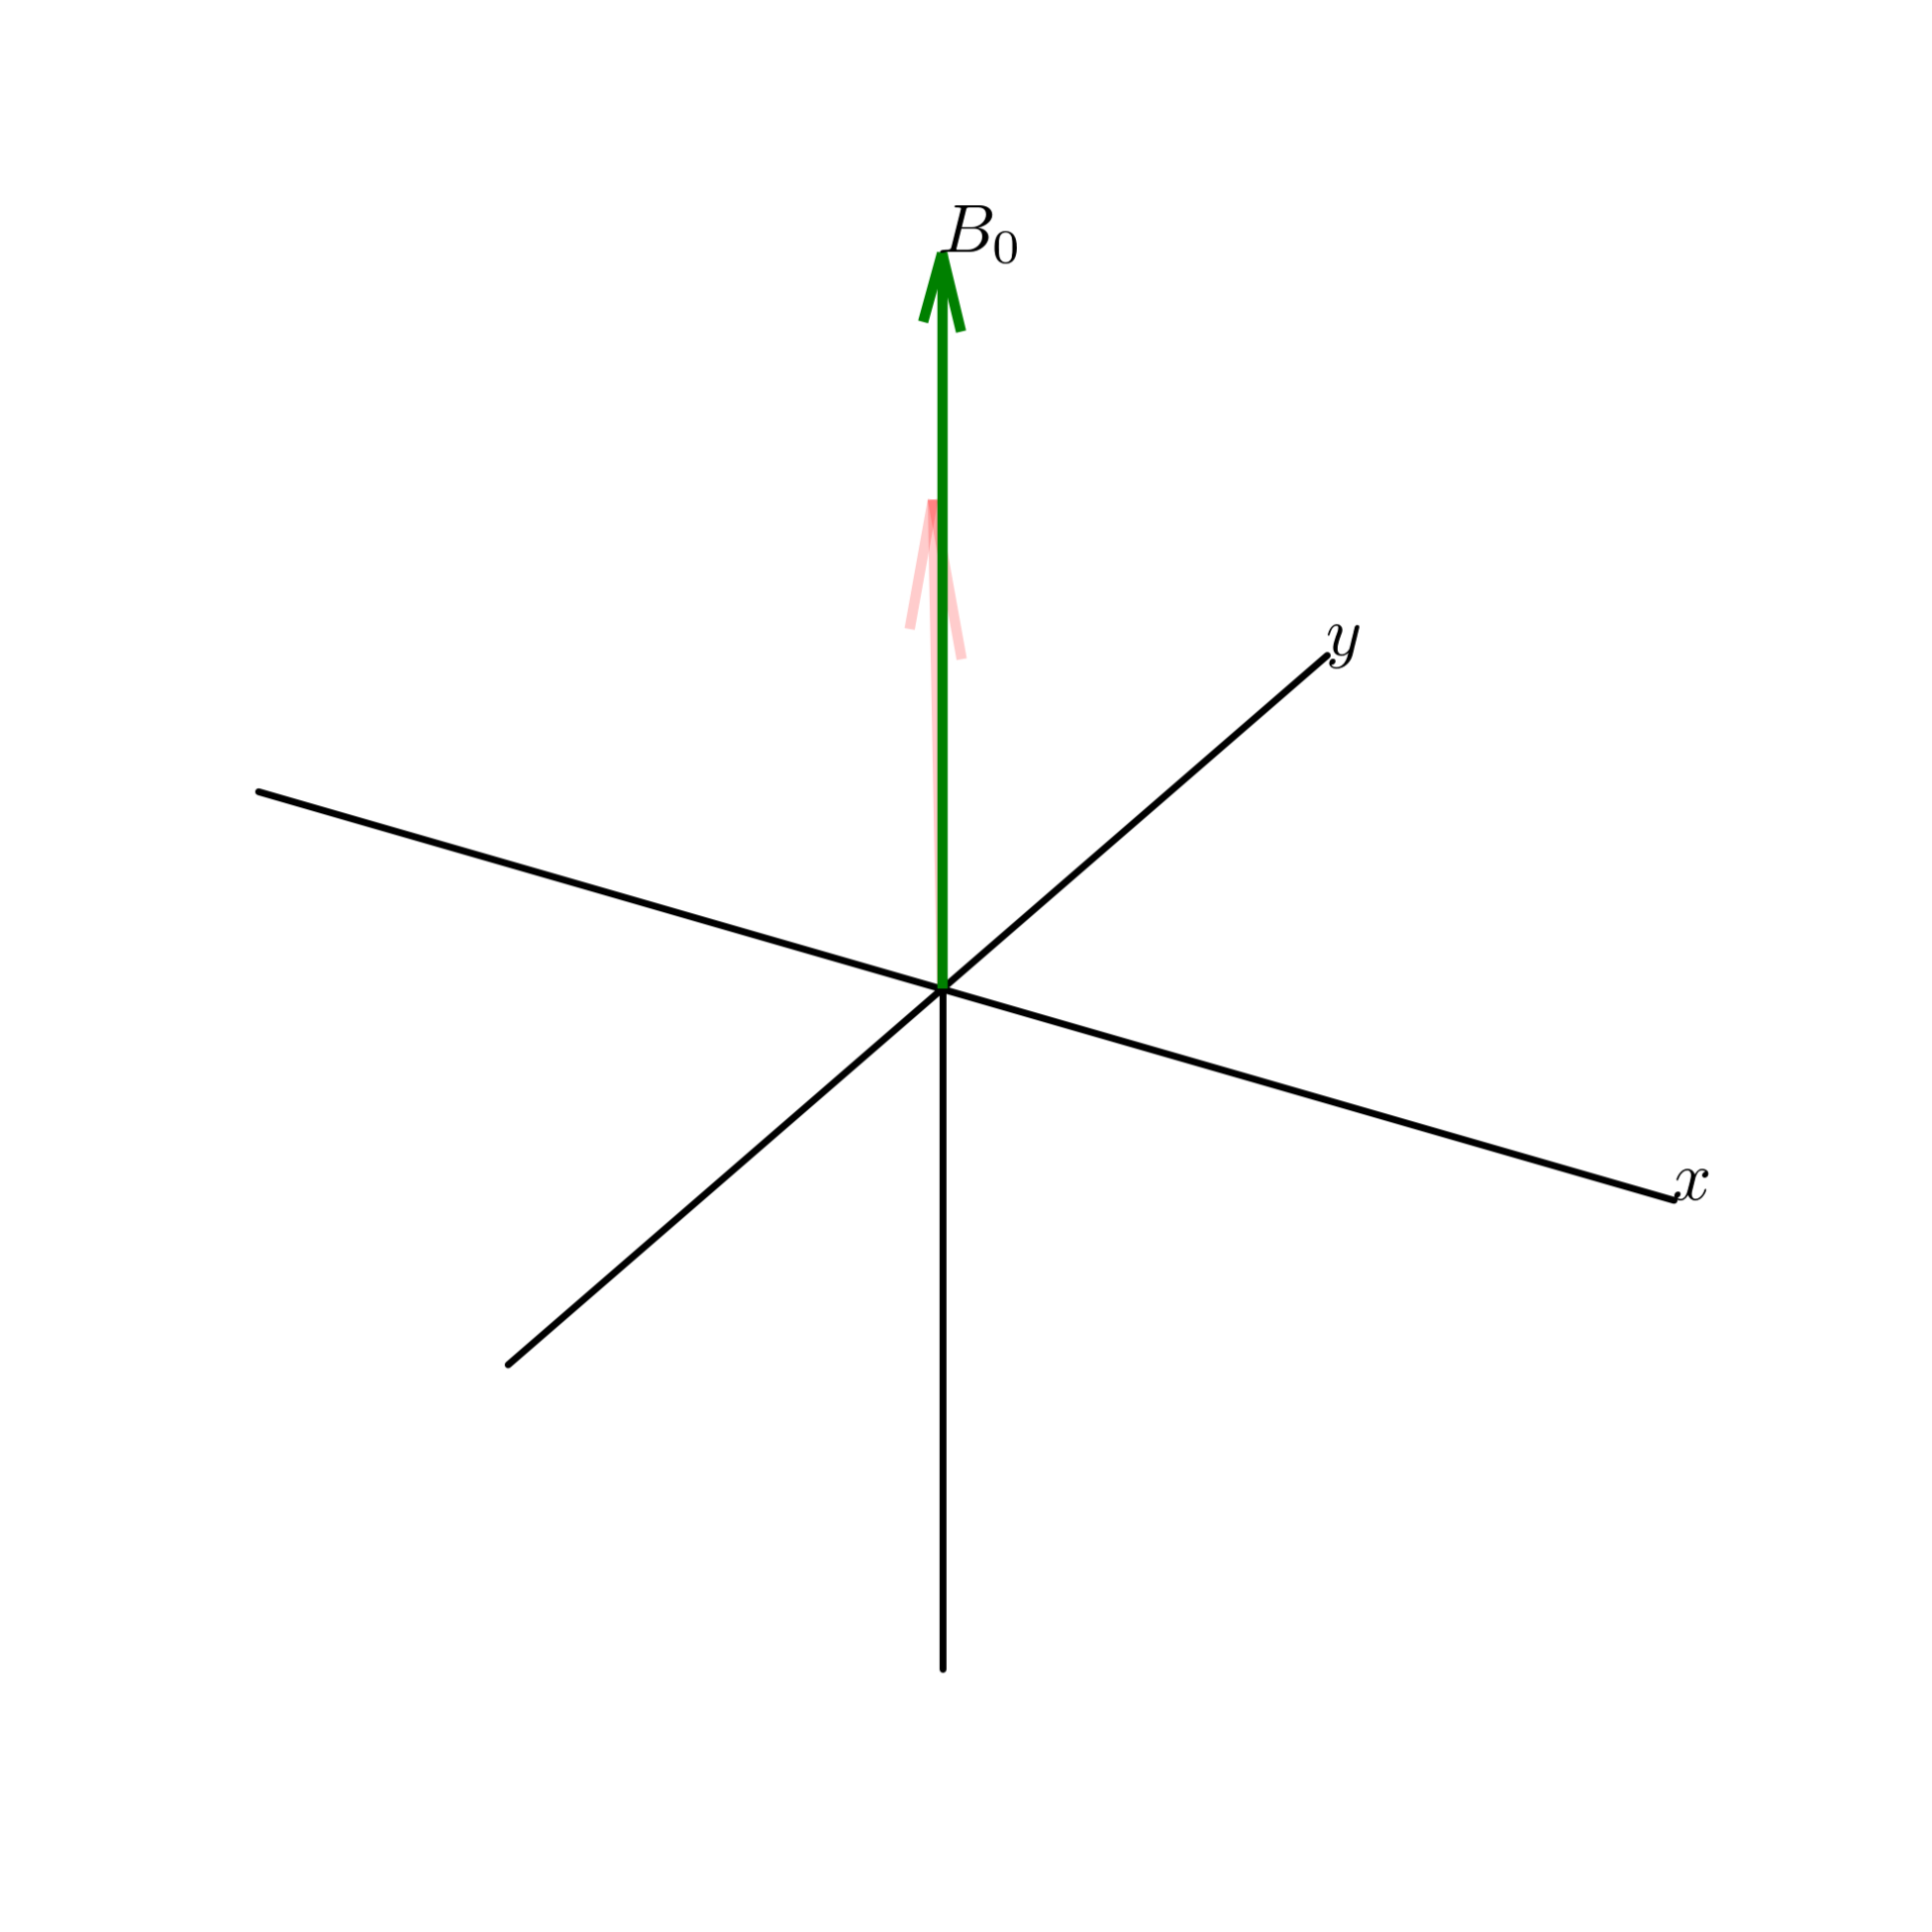
\includegraphics[width = 0.4\linewidth]{setup.png}\\
    %             {\small Typical $\Bnot$ and vector aligned with field}
    %     \end{tabular}
    %     & \begin{tabular}{l}
    %         \parbox{0.25\linewidth}{
    %             \begin{itemize}
    %                 \item Spin \half nuclei 
    %                 \item Strong magnetic field, denoted $\Bnot$
    %             \end{itemize}
    %         }\\

    %         \begin{block}{Energy and Hamiltonian}
    %             \begin{equation}
    %                 E = -\vec{\mu} \cdot \vec{B_0}
    %             \end{equation}
    %         \end{block}
    %     \end{tabular}
    % \end{tabular}
\end{frame}

%------------------------------------------------

\begin{frame}{Larmor Precession}

    \begin{minipage}{0.6\linewidth}
        Evolving an arbitrary spin vector
        \begin{gather*}
            \ket{\psi} = \cos\left(\sfrac{\theta}{2}\right)\ket{+}+ e^{i\phi}\sin\left(\sfrac{\theta}{2}\right) \ket{-}
        \end{gather*}
        yields, 
        \begin{align*}
            \langle S_x \rangle &= \frac{\hbar}{2} \sin(\theta)\cos(\gamma B_0 t)\\
            \langle S_y \rangle &= \frac{\hbar}{2} \sin(\theta)\sin(\gamma B_0 t)\\
            \langle S_z \rangle &= \frac{\hbar}{2} \cos(\theta)   
        \end{align*}
        with the characteristic \textbf{Larmor frequency}
        \begin{equation}
            \omega_0 = \gamma B_0 
        \end{equation}
    \end{minipage}
    \begin{minipage}{0.3\linewidth}
        % IF YOU WANT THE HAMILTONIAN AND EIGENSTATES COME BACK HERE % 
        % \begin{block}{Hamiltonian of System}
        %     \begin{equation}\label{eqn:hamiltonian}
        %         H = -\frac{\hbar}{2} \gamma B_0  \pauliz
        %     \end{equation}
        %     with eigenstates
        %     \begin{equation}
        %         \ket{\pm} : E_\pm = \mp \frac{\hbar}{2} \gamma B_0 
        %     \end{equation}        
        % \end{block}

        
    \end{minipage}
    
\end{frame}


%------------------------------------------------

\begin{frame}{Blocks of Highlighted Text}
    In this slide, some important text will be \alert{highlighted} because it's important. Please, don't abuse it.

    \begin{block}{Block}
        Sample text
    \end{block}

    \begin{alertblock}{Alertblock}
        Sample text in red box
    \end{alertblock}

    \begin{examples}
        Sample text in green box. The title of the block is ``Examples".
    \end{examples}
\end{frame}

%------------------------------------------------

\begin{frame}{Multiple Columns}
    \begin{columns}[c] % The "c" option specifies centered vertical alignment while the "t" option is used for top vertical alignment

        \column{.45\textwidth} % Left column and width
        \textbf{Heading}
        \begin{enumerate}
            \item Statement
            \item Explanation
            \item Example
        \end{enumerate}

        \column{.45\textwidth} % Right column and width
        Lorem ipsum dolor sit amet, consectetur adipiscing elit. Integer lectus nisl, ultricies in feugiat rutrum, porttitor sit amet augue. Aliquam ut tortor mauris. Sed volutpat ante purus, quis accumsan dolor.

    \end{columns}
\end{frame}

%------------------------------------------------
\section{Second Section}
%------------------------------------------------

\begin{frame}{Table}
    \begin{table}
        \begin{tabular}{l l l}
            \toprule
            \textbf{Treatments} & \textbf{Response 1} & \textbf{Response 2} \\
            \midrule
            Treatment 1         & 0.0003262           & 0.562               \\
            Treatment 2         & 0.0015681           & 0.910               \\
            Treatment 3         & 0.0009271           & 0.296               \\
            \bottomrule
        \end{tabular}
        \caption{Table caption}
    \end{table}
\end{frame}

%------------------------------------------------

\begin{frame}{Theorem}
    \begin{theorem}[Mass--energy equivalence]
        $E = mc^2$
    \end{theorem}
\end{frame}

%------------------------------------------------

\begin{frame}{Figure}
    Uncomment the code on this slide to include your own image from the same directory as the template .TeX file.
    %\begin{figure}
    %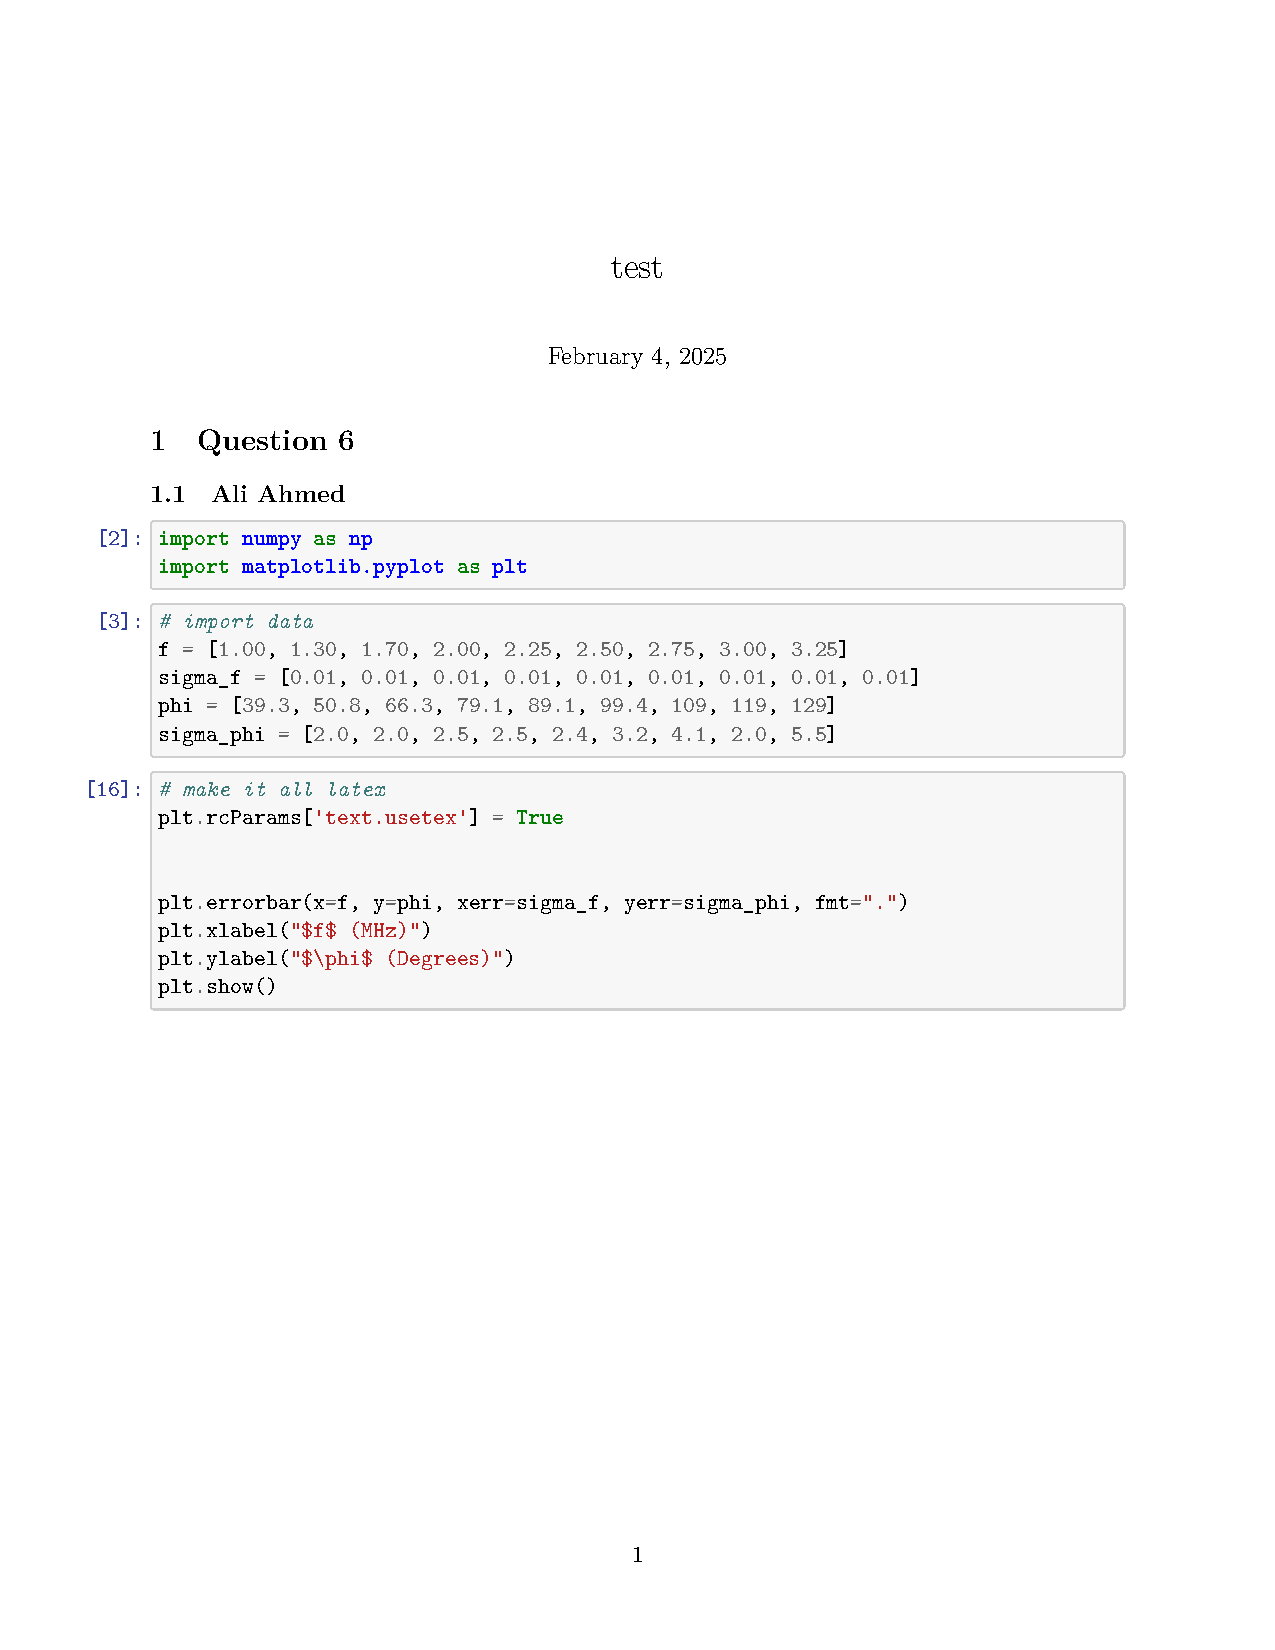
\includegraphics[width=0.8\linewidth]{test}
    %\end{figure}
\end{frame}

%------------------------------------------------

\begin{frame}[fragile] % Need to use the fragile option when verbatim is used in the slide
    \frametitle{Citation}
    An example of the \verb|\cite| command to cite within the presentation:\\~

    This statement requires citation \cite{p1}.
\end{frame}

%------------------------------------------------

\begin{frame}{References}
    \footnotesize
    \bibliography{reference.bib}
    \bibliographystyle{apalike}
\end{frame}

%------------------------------------------------

\begin{frame}
    \Huge{\centerline{\textbf{The End}}}
\end{frame}

%----------------------------------------------------------------------------------------

\end{document}